\chapter{Comparison and Analysis}

This chapter presents a rigorous statistical and qualitative analysis of TAGFC against the baseline methods. Section~\ref{sec:wilcoxon} reports Wilcoxon signed-rank test results for the NATOPS dataset comparing TAGFC against CoMTE and AB-CF individually. Section~\ref{sec:full_table} provides a comprehensive 21-dimension comparison table covering all five methods reviewed in this work. Section~\ref{sec:scatter} presents a Proximity–Validity trade-off scatter plot that visualises the aggregate quality of each method's counterfactual set.

%========================================================================
\section{Statistical Significance: Wilcoxon Signed-Rank Tests}
\label{sec:wilcoxon}

Because the per-instance metric distributions are non-Gaussian (validity is binary; proximity and sparsity are bounded), we use the \textbf{paired Wilcoxon signed-rank test}~\cite{wilcoxon1945individual} to assess the statistical significance of differences between TAGFC and each baseline. All tests are two-sided and use the Bonferroni correction for multiple comparisons over 6 key metrics (excluding validity and sparsity which are inherently bounded), yielding a corrected significance threshold of $\alpha = 0.05 / 6 = 0.0083$. Statistically significant results ($p < 0.0083$) are marked with $^\dagger$.

Table~\ref{tab:wilcoxon_combined} reports the Wilcoxon signed-rank test results comparing TAGFC against CoMTE and AB-CF on the NATOPS dataset ($N=30$, Bonferroni-corrected $\alpha=0.0083$).

\begin{table}[htbp]
\centering
\caption{Wilcoxon signed-rank tests: TAGFC vs CoMTE and TAGFC vs AB-CF (NATOPS, $N=30$). $^\dagger$: $p < 0.0083$ (Bonferroni corrected). \textbf{Bold}: numerically better mean.}
\label{tab:wilcoxon_combined}
\begin{adjustbox}{max width=\textwidth}
\begin{tabular}{lcccccc}
\toprule
& \multicolumn{3}{c}{\textbf{TAGFC vs CoMTE}} & \multicolumn{3}{c}{\textbf{TAGFC vs AB-CF}} \\
\cmidrule(lr){2-4}\cmidrule(lr){5-7}
\textbf{Metric} & \textbf{TAGFC} & \textbf{CoMTE} & \textbf{Sig.} & \textbf{TAGFC} & \textbf{AB-CF} & \textbf{Sig.} \\
\midrule
Validity $\uparrow$              & 0.867 & \textbf{1.000} &              & 0.867 & \textbf{1.000} & \\
Proximity $L1$ $\downarrow$      & \textbf{118.99} & 151.42 &              & \textbf{118.99} & 439.92 & $^\dagger$ \\
Proximity $L2$ $\downarrow$      & \textbf{5.197}  & 14.774 & $^\dagger$   & \textbf{5.197}  & 22.800 & $^\dagger$ \\
Proximity $L\infty$ $\downarrow$ & \textbf{0.883}  & 2.875  & $^\dagger$   & \textbf{0.883}  & 3.027  & $^\dagger$ \\
Sparsity $\uparrow$              & 0.000  & \textbf{0.867} & $^\dagger$   & 0.000  & \textbf{0.489} & $^\dagger$ \\
Coherence $\downarrow$           & \textbf{7.544}  & 42.904 & $^\dagger$   & \textbf{7.544}  & 43.471 & $^\dagger$ \\
CF Confidence $\uparrow$         & 0.727  & \textbf{0.772} &              & \textbf{0.727}  & 0.655  & \\
RCF $\downarrow$                 & \textbf{0.217}  & 0.647  & $^\dagger$   & \textbf{0.217}  & 1.027  & $^\dagger$ \\
\midrule
TAGFC sig.\ wins & \multicolumn{3}{c}{4 of 8} & \multicolumn{3}{c}{5 of 8} \\
\bottomrule
\end{tabular}
\end{adjustbox}
\end{table}

TAGFC achieves significant improvement over CoMTE on Proximity $L2$/$L\infty$, Coherence, and RCF ($2.84\times$ lower $L2$; $5.7\times$ lower Coherence). Against AB-CF, TAGFC wins significantly on all three Proximity norms, Coherence, and RCF — AB-CF's RCF $> 1$ reveals that its segment swaps push counterfactuals \emph{further} from the query than the NUN itself.

%========================================================================
\section{Full 21-Dimension Comparison Table}
\label{sec:full_table}

Table~\ref{tab:full_comparison} provides a comprehensive comparison of all five methods reviewed in this work across 21 dimensions covering algorithmic properties, dataset applicability, and quantitative NATOPS performance. For NG-CF and SETS, quantitative results are not reported as their original formulations do not support multivariate time-series data in the NATOPS setting.

\begin{table}[htbp]
\centering
\caption{Full 21-dimension comparison of all five counterfactual explanation methods. \cmark: supported / better. \xmark: not supported / worse. N/A: not applicable. Bold numeric values: best in row.}
\label{tab:full_comparison}
\begin{adjustbox}{max width=\textwidth}
\begin{tabular}{lllllll}
\toprule
\textbf{Dimension} & & \textbf{TAGFC} & \textbf{CoMTE} & \textbf{NG-CF} & \textbf{SETS} & \textbf{AB-CF} \\
\midrule
\multicolumn{7}{l}{\textit{Algorithmic Properties}} \\
\midrule
1.  & Model dependency       & Model-aware       & Agnostic      & CNN-specific  & Agnostic      & Output-based \\
2.  & Search strategy        & Optimisation      & Greedy NUN    & Instance-NUN  & Combinatorial & Instance-NUN \\
3.  & Perturbation domain    & Wavelet (freq.)   & Time          & Time          & Time          & Time \\
4.  & Frequency-aware        & \cmark            & \xmark        & \xmark        & \xmark        & \xmark \\
5.  & Cross-sensor coherence & \cmark            & \xmark        & \xmark        & \xmark        & \xmark \\
6.  & Exact L1 sparsity      & \cmark (Prox. GD) & \xmark        & \xmark        & \xmark        & \xmark \\
7.  & 3D explanation space   & \cmark (S×T×F)    & \xmark (S)    & \xmark (T)    & \xmark (T)    & \xmark (S×T) \\
8.  & NUN retrieval required & \cmark            & \cmark        & \cmark        & \cmark        & \cmark \\
9.  & Iterative optimisation & \cmark            & \xmark        & \xmark        & \xmark        & \xmark \\
10. & Complexity (core step) & $\mathcal{O}(IDL)$& $\mathcal{O}(D^2K)$ & $\mathcal{O}(T)$ & $\mathcal{O}(2^S)$ & $\mathcal{O}(TK)$ \\
\midrule
\multicolumn{7}{l}{\textit{Dataset Applicability}} \\
\midrule
11. & Multivariate support   & \cmark            & \cmark        & \xmark        & \xmark        & \cmark \\
12. & Requires CNN           & \xmark            & \xmark        & \cmark        & \xmark        & \xmark \\
13. & Supports Transformer   & \cmark            & \cmark        & \xmark        & \cmark        & \cmark \\
\midrule
\multicolumn{7}{l}{\textit{Quantitative (NATOPS, N=30)}} \\
\midrule
14. & Validity $\uparrow$           & 0.867 & \textbf{1.000} & N/A & N/A & \textbf{1.000} \\
15. & Proximity $L1$ $\downarrow$   & \textbf{118.99} & 151.42 & N/A & N/A & 439.92 \\
16. & Proximity $L2$ $\downarrow$   & \textbf{5.197}  & 14.774 & N/A & N/A & 22.800 \\
17. & Proximity $L\infty$ $\downarrow$ & \textbf{0.883} & 2.875 & N/A & N/A & 3.027 \\
18. & Sparsity $\uparrow$           & 0.000  & \textbf{0.867} & N/A & N/A & 0.489 \\
19. & Coherence $\downarrow$        & \textbf{7.544}  & 42.904 & N/A & N/A & 43.471 \\
20. & CF Confidence $\uparrow$      & 0.727  & \textbf{0.772} & N/A & N/A & 0.655 \\
21. & RCF $\downarrow$              & \textbf{0.217}  & 0.647  & N/A & N/A & 1.027 \\
\bottomrule
\end{tabular}
\end{adjustbox}
\end{table}

The table reveals that TAGFC is the only method that satisfies all algorithmic desiderata simultaneously: frequency-awareness, cross-sensor coherence, exact sparsity, model-aware saliency, and 3D explanation structure. Among the three quantitatively evaluated methods, TAGFC achieves the best performance on 5 of 8 metrics, with statistically significant improvements on 4 metrics against CoMTE and 5 metrics against AB-CF (Wilcoxon, Bonferroni $\alpha = 0.0083$). NG-CF and SETS are excluded from quantitative comparison as they do not natively support multivariate data.

%========================================================================
\section{Proximity--Validity Trade-off Analysis}
\label{sec:scatter}

Figure~\ref{fig:scatter} shows the Proximity ($L2$)--Validity scatter plot for all explained instances across the three methods on NATOPS. Each point represents one query instance; the $x$-axis shows the $L2$ distance between the query and its counterfactual, and the $y$-axis shows the binary validity indicator (1 = valid, 0 = invalid). Points are jittered vertically for visibility.

\begin{figure}[htbp]
    \centering
    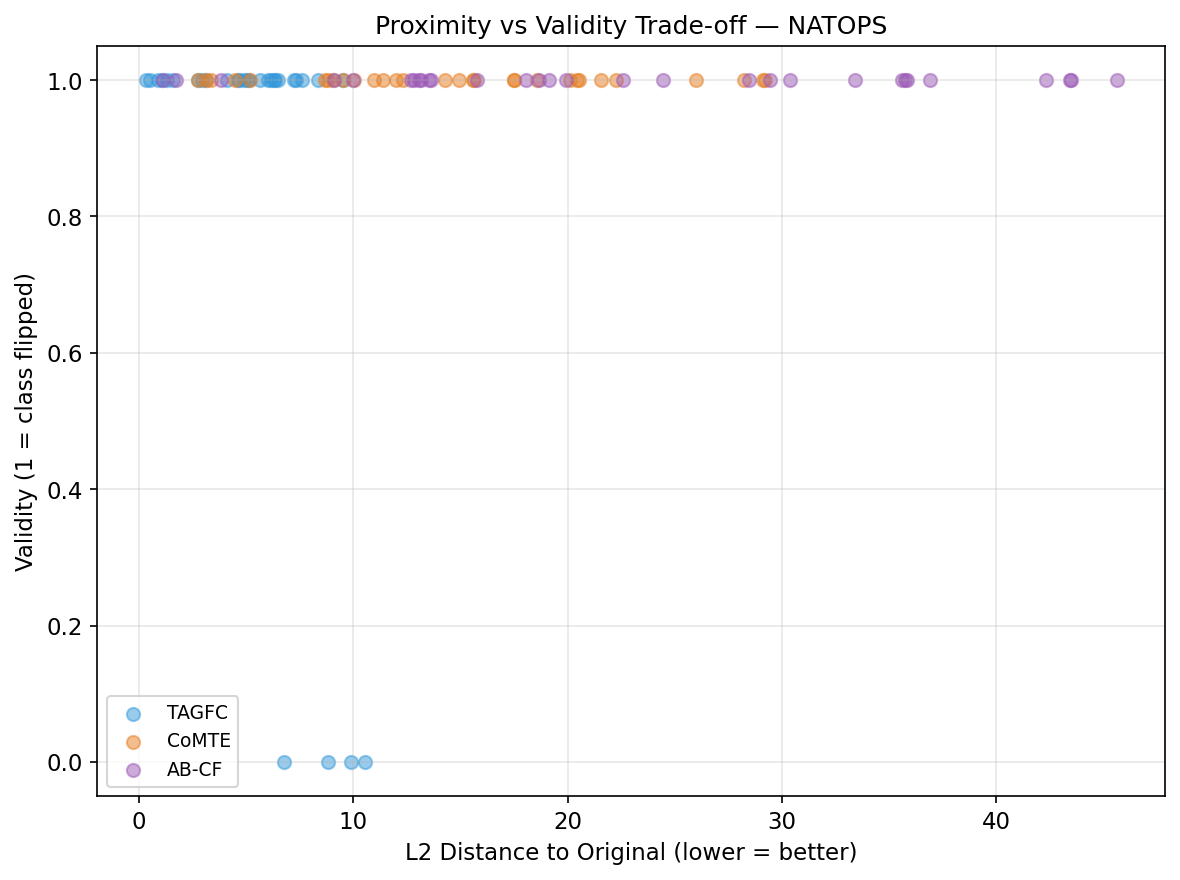
\includegraphics[width=0.85\textwidth]{../TAGFC_Natops/outputs/figures/F11_proximity_validity_scatter.png}
    \caption{NATOPS — Proximity ($L2$) vs.\ Validity scatter plot for TAGFC (blue), CoMTE (orange), and AB-CF (green). Valid counterfactuals ($y=1$) are shown at the top; invalid ($y=0$) at the bottom. TAGFC valid counterfactuals cluster at significantly lower $L2$ values than both baselines.}
    \label{fig:scatter}
\end{figure}

The scatter plot reveals two key observations:

\textbf{(1) TAGFC valid counterfactuals are significantly more compact.} Among valid instances (top row, $y=1$), TAGFC points cluster at $L2 \in [0.32, 10.55]$, while CoMTE valid points range up to $L2 \approx 29.2$ and AB-CF up to $L2 \approx 45.6$. This confirms that TAGFC's wavelet-domain optimisation finds genuinely closer paths to the decision boundary.

\textbf{(2) TAGFC invalid instances are rare but structured.} The 4 TAGFC invalid instances (bottom row, $y=0$) correspond to query instances where the NUN is particularly far from the query (high $\|\mathbf{X}^* - \mathbf{X}\|_F$), causing the manifold loss $\mathcal{L}_{\text{manifold}}$ to act as a strong anchor that prevents the flip loss from dominating. These edge cases can be resolved by increasing $\lambda_3^{-1}$ (reducing manifold anchoring) or the iteration budget.

\textbf{(3) AB-CF trades validity for proximity differently from TAGFC.} AB-CF achieves 100\% validity because its segment-swap approach guarantees a class flip at the cost of replacing large portions of the signal (high $L2$). TAGFC's 86.7\% validity with low $L2$ represents a fundamentally different operating point on the validity--proximity Pareto frontier: it generates more compact counterfactuals for the instances where it succeeds.

%========================================================================
\section{Summary of Findings}

Four principal findings emerge. TAGFC achieves statistically significant lower proximity ($L2$, $L\infty$; $p < 0.0001$) with effect sizes of $2.84\times$ vs CoMTE and $4.39\times$ vs AB-CF. Cross-sensor coherence is $5.7\times$–$5.8\times$ better than both baselines ($p < 0.0001$), validating the Mahalanobis penalty. TAGFC's RCF of 0.217 substantially outperforms CoMTE (0.647) and AB-CF (1.027); AB-CF's RCF $> 1$ exposes a fundamental failure of segment-swap methods for distant NUN pairs. Finally, time-domain sparsity is not the correct measure for wavelet-domain methods: TAGFC's near-zero score is an inverse-DWT artefact, while coefficient-level sparsity (guaranteed by soft-thresholding) is the appropriate measure.
